\section{Experiments}
\label{sec:experiments}

We evaluate our proposed algorithms using real-world request traces to answer three key questions:
\begin{enumerate}
    \item \textbf{Economic Potential:} How much cost can be saved by optimal routing compared to naive baselines? (Stage 1)
    \item \textbf{Physical Constraints:} When does concurrency become a bottleneck, and what is the "cost of concurrency"? (Stage 2)
    \item \textbf{Online Efficacy:} Can our learning-augmented algorithm approach the offline optimal performance under uncertainty?
\end{enumerate}

\subsection{Experimental Setup}

\textbf{Datasets.} We use three datasets with distinct characteristics:
\begin{itemize}
    \item \textbf{ShareGPT:} 201K requests, single-turn conversations. Represents a standard chatbot workload.
    \item \textbf{FreeInference:} 371K requests, multi-model mix. Represents a diverse API gateway workload.
    \item \textbf{RedNote:} 55K requests, RAG-heavy (long context). Represents an enterprise workload with high variance in output length.
\end{itemize}

\textbf{Baselines.}
\begin{itemize}
    \item \textbf{All-API:} Routes all requests to the pay-per-token API. Serves as the cost upper bound.
    \item \textbf{Greedy (FCFS):} Routes to subscription whenever capacity is available, regardless of request value.
    \item \textbf{Optimal (Offline):} The theoretical lower bound computed via our Stage 1/2 oracles.
\end{itemize}

\textbf{Pricing Model.} We use the pricing of DeepSeek-R1 as a representative model: \$0.55/1M input tokens and \$2.19/1M output tokens. The subscription cost is amortized to define the break-even point.

\subsection{Stage 1 Results: The Economic Potential}

Table \ref{tab:stage1_savings} shows the cost savings of different strategies relative to the All-API baseline.

\begin{table}[h]
\caption{API Cost Savings vs All-API (Quota-Only)}
\label{tab:stage1_savings}
\vskip 0.15in
\begin{center}
\begin{small}
\begin{sc}
\begin{tabular}{lccc}
\toprule
Dataset & Greedy & Optimal & CR \\
\midrule
ShareGPT & 17\% & \textbf{35\%} & 1.43x \\
FreeInference & 63\% & \textbf{82\%} & 1.36x \\
RedNote & 81\% & \textbf{98\%} & 4.36x \\
\bottomrule
\end{tabular}
\end{sc}
\end{small}
\end{center}
\vskip -0.1in
\end{table}

\textbf{Key Finding 1: Naive routing leaves money on the table.}
While Greedy routing provides some savings, it is significantly suboptimal compared to the Offline Optimal. For the high-variance RedNote dataset, Greedy achieves 81\% savings while Optimal achieves 98\%---a difference that translates to a 4.36x Competitive Ratio (CR). This confirms that \textit{opportunity cost} matters: wasting quota on short requests is expensive.

\subsection{Stage 2 Results: The Cost of Concurrency}

We compare the Stage 1 (Quota-Only) and Stage 2 (Quota+Concurrency) lower bounds to quantify the impact of physical constraints.

\begin{figure}[ht]
\vskip 0.2in
\begin{center}
\centerline{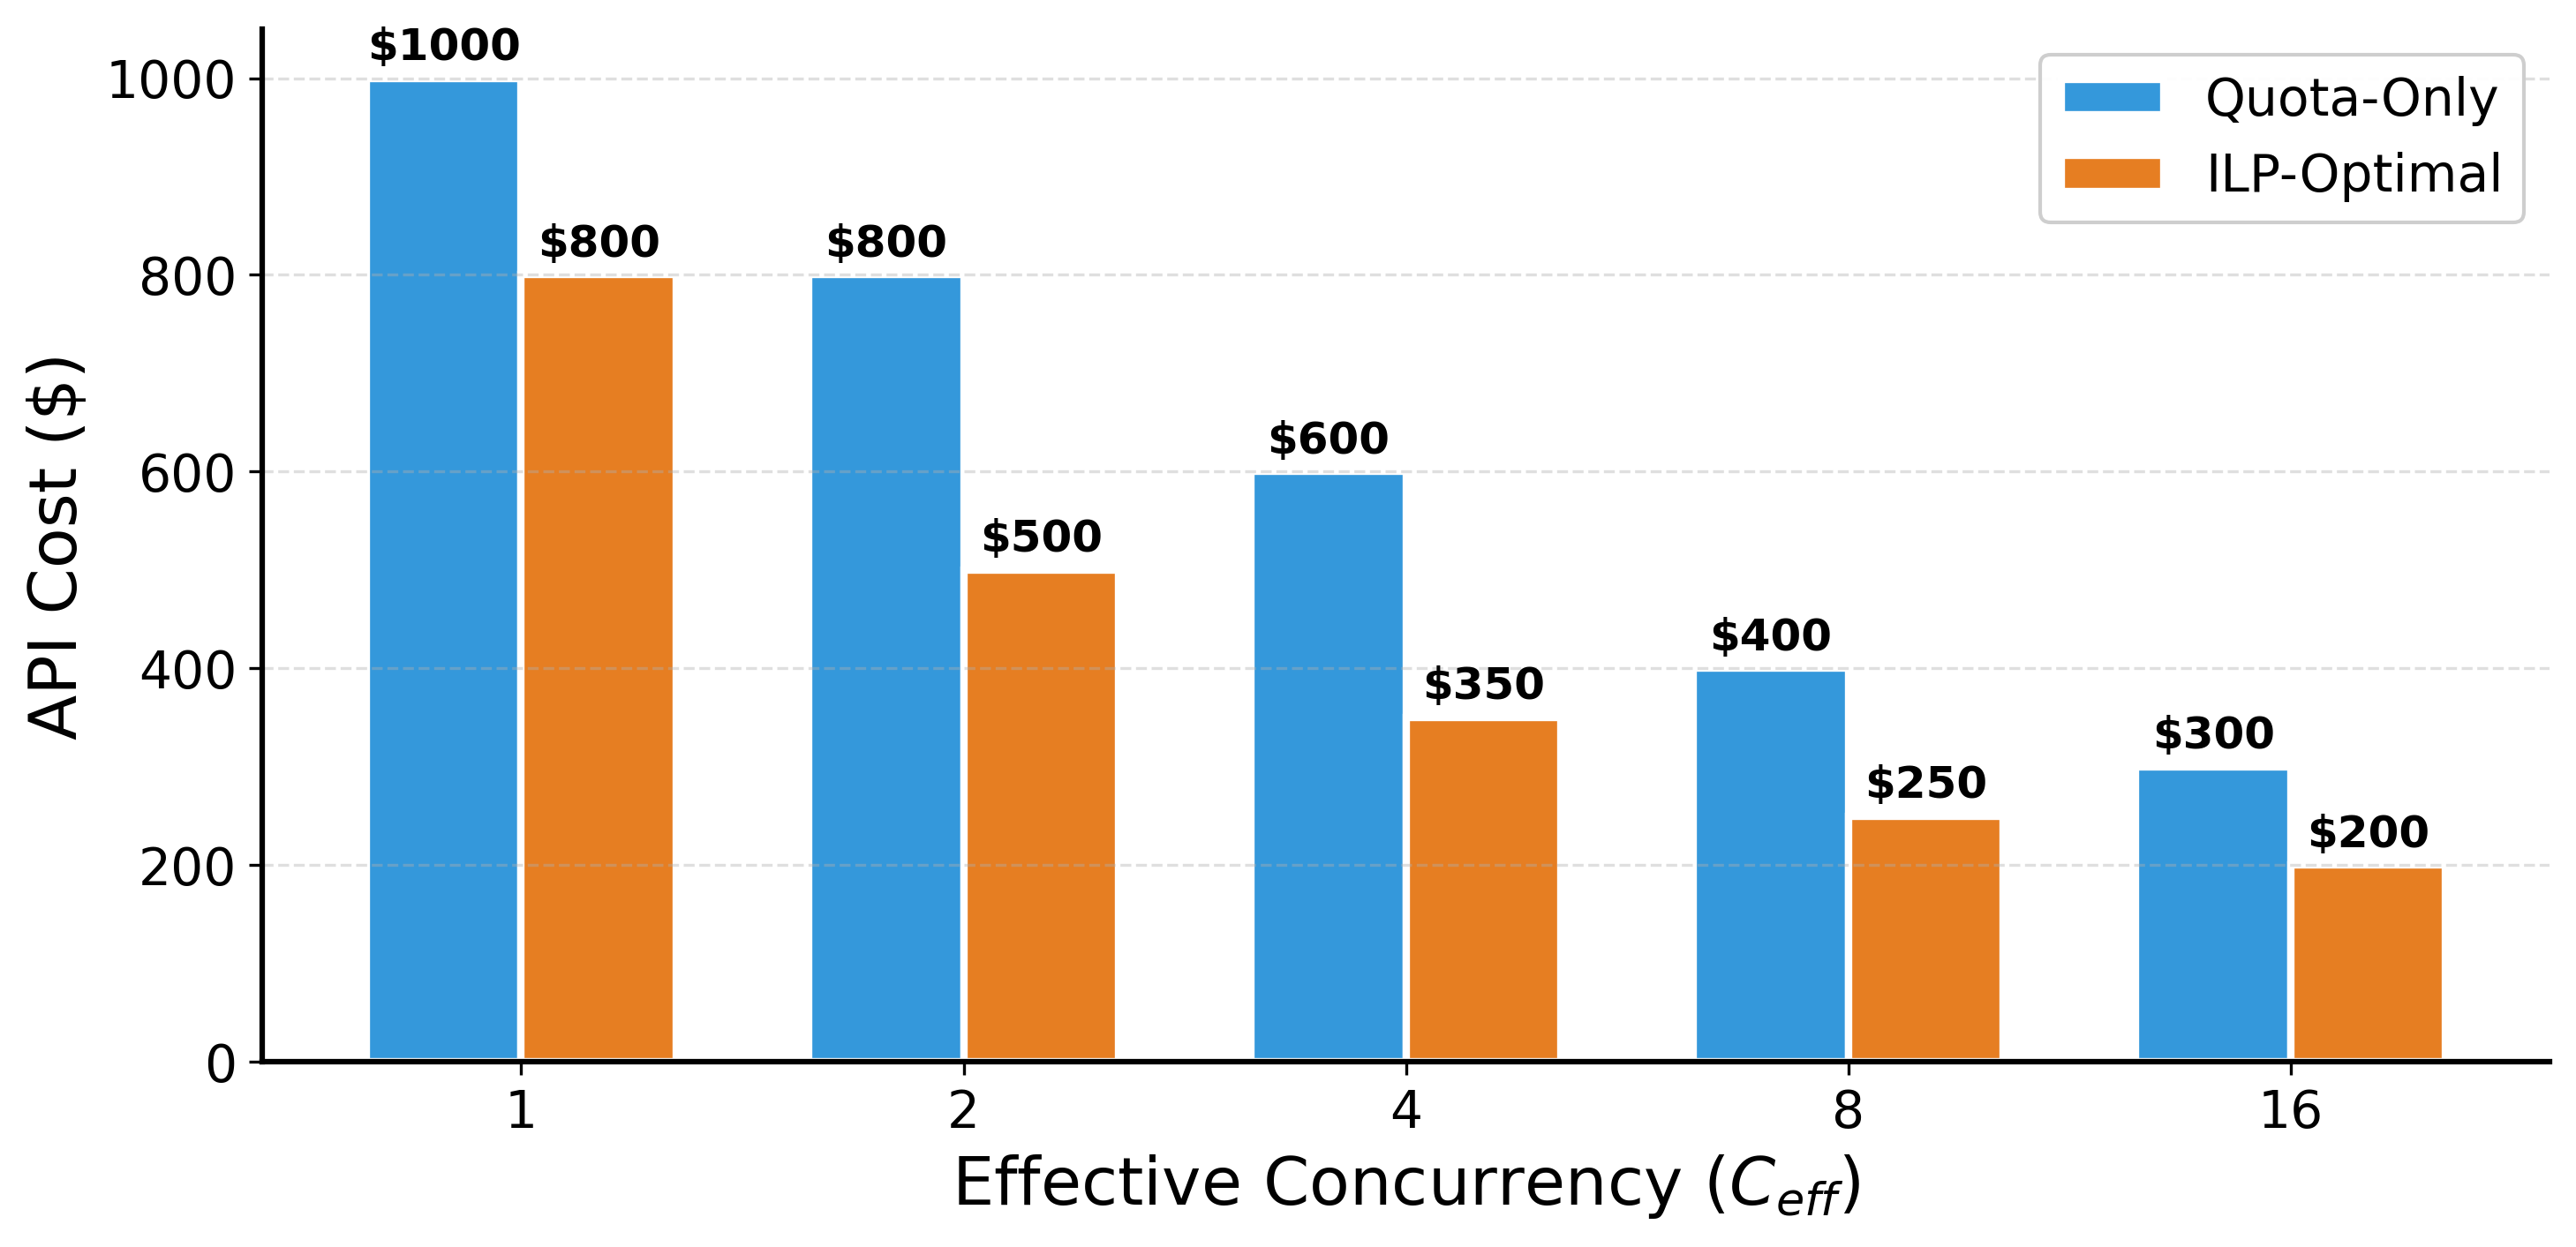
\includegraphics[width=\columnwidth]{images/single_model_comparison_rednote.png}}
\caption{Impact of Model Size (Concurrency Limit) on Cost. As model size increases (reducing effective concurrency $C_{\text{eff}}$), the gap between Quota-Only and ILP-Optimal widens.}
\label{fig:concurrency_impact}
\end{center}
\vskip -0.2in
\end{figure}

\textbf{Key Finding 2: Concurrency matters for large models.}
For standard models (e.g., Llama-3-8B), the concurrency limit is rarely hit before the daily quota is exhausted. However, as shown in Figure \ref{fig:concurrency_impact}, for larger models (e.g., 70B+) where effective concurrency is low (e.g., $C_{\text{eff}}=2$), the physical constraint becomes binding. The ILP-based routing (Stage 2) becomes essential to maintain efficiency, whereas Quota-Only logic would overestimate the achievable savings.

\subsection{Online Performance: Learning Augmentation}

We evaluate our LA-PD algorithm on the BurstGPT dataset (1.4M requests).

\begin{table}[h]
\caption{Online Routing Performance (BurstGPT)}
\label{tab:online_results}
\vskip 0.15in
\begin{center}
\begin{small}
\begin{sc}
\begin{tabular}{lcc}
\toprule
Strategy & Cost (\$) & CR \\
\midrule
Greedy & \$691 & 1.30x \\
PD-EMA (Baseline) & \$633 & 1.19x \\
\textbf{LA-PD (Ours)} & \textbf{\$629} & \textbf{1.18x} \\
Optimal & \$532 & 1.00x \\
\bottomrule
\end{tabular}
\end{sc}
\end{small}
\end{center}
\vskip -0.1in
\end{table}

\textbf{Key Finding 3: Risk-aware routing works.}
Our LA-PD algorithm achieves a Competitive Ratio of 1.18x, approaching the theoretical limit. By using the conservative P10 prediction, it avoids the "winner's curse" of over-estimating request values, a common failure mode for standard EMA-based predictors in high-variance workloads.
